% !TEX root = ../axiomatic.tex

\section{Proof}\label{s:proof}

In this section we present the proof of our main theorem: any \mbox{cup-$i$} construction that is non-degenerate, irreducible and free is isomorphic to the canonical one.
We divide this proof into several parts.
In \cref{ss:properties} we revisit the axioms defining our characterization in light of the previous section.
A useful consequence of freeness is recorded in \cref{ss:consequence}.
The base case of an induction argument is given in \cref{ss:cases}; whereas in
\cref{ss:fact} we recall a fact about our presentation of the canonical cup-$i$ construction.
We devote \cref{ss:preparing} to prepare an induction step and \cref{ss:step} to present it.
Our theorem is finally proven in \cref{ss:proof} using the foreshadowed induction argument.

\subsection{Axioms revisited}\label{ss:properties}

We start by recasting the axioms introduced in \cref{d:properties} using the reformulation of the previous section and observe that the canonical cup-$i$ construction satisfies them.

\begin{lemma}\label{l:properties}
	Consider for each $i,n \in \N$ an element
	\[
	\triangle_i [n] =
	\sum_{\mathclap{\lambda \in \Lambda(i,n)}} V_\lambda \ot W_\lambda
	\]
	with each $V_\lambda \ot W_\lambda$ in the basis of $\cP(\simplex^n)^{\ot 2}_{i+n}$.
	Assume $\big\{ \triangle_i [n] \big\}_{i,n \in \N}$ defines a \mbox{cup-$i$} construction, then:
	\begin{enumerate}
		\item It is non-degenerate iff
		$\triangle_0 [0] \neq 0$.
		\item It is irreducible iff\,
		$\forall i,n \in \N$, $\forall \lambda \in \Lambda(i,n)$, $V_\lambda \cap W_\lambda = \emptyset$.
		\item \label{i:free} It is free iff\,
		$\forall i,n \in \N$, $\forall \lambda_1, \lambda_2 \in \Lambda(i,n)$, $V_{\lambda_1} \ot W_{\lambda_1} \neq W_{\lambda_2} \ot V_{\lambda_2}$ if $i \neq n$.
	\end{enumerate}
\end{lemma}

\begin{proof}
	By naturality, it suffices to verify these equivalences for the \mbox{cup-$i$} product structure defined on $\cochains(X)$ when $X = \simplex^n$ for every $n \in \N$.
	We will use the fact that the isomorphism $\Psi_n^{\ot 2} \colon \cP(\gsimplex)^{\ot 2} \to \chains(\gsimplex^2)^{\ot 2}$ sends basis elements to basis elements, as does the linear duality isomorphism between chains and cochains.

	\noindent (1) To prove this equivalence it suffices to assume $n = 0$ by naturality.
	Then the statement follows from the fact that $\cochains(\gsimplex^0)^{\ot 2}$ is one dimensional.

	\noindent (2) To prove this equivalence notice that there is $k \in V_\lambda \cap W_\lambda$ for one of the summands of $\triangle_i [n]$ if an only the image of this summand under $\Psi_n^{\ot 2}$ is
	\[
	\underbrace{d_{V_\lambda \setminus k} \overbrace{d_k[n]}^{y}}_{y^{(1)}}
	\ot
	\underbrace{d_{W_\lambda \setminus k} \overbrace{d_k[n]}^{y}}_{y^{(2)}}
	\]
	with $y^{(1)} \smallsmile_i y^{(2)} \neq 0$.

	\noindent (3) This equivalence follows directly from considering the isomorphism $\Psi_n^{\ot 2}$.
\end{proof}

The following is deduced from \cref{l:properties} by inspecting \cref{l:canonical}.

\begin{theorem}\label{t:existence}
	The canonical \mbox{cup-$i$} construction is non-degenerate, irreducible, and free.
\end{theorem}

\subsection{A consequence of freeness}\label{ss:consequence}

We record an important observation concerning free cup-$i$ constructions.

\begin{lemma}\label{l:consequence}
	Let $\big\{ \triangle_i [n] \big\}_{i,n\in\N}$ be a free \mbox{cup-$i$} construction.
	If
	\[
	(1+T) \triangle_i [n] =
	(1+T) \sum_{\mathclap{\lambda \in \Lambda(i,n)}} V_\lambda \ot W_\lambda
	\]
	for $i,n \in \N$ with $i \neq n$ and each $V_\lambda \ot W_\lambda$ is a basis element of $\cP(\simplex^n)^{\ot 2}_{i+n}$, then there is a partition of $\Lambda(i,n) = \Lambda_1 \sqcup \Lambda_2$ with
	\begin{equation}\label{e:splitting}
	\triangle_i [n] =
	\sum_{\lambda_1 \in \Lambda_1} V_{\lambda_1} \ot W_{\lambda_1} \, +
	\sum_{\lambda_2 \in \Lambda_2} W_{\lambda_2} \ot V_{\lambda_2}.
	\end{equation}
\end{lemma}

\begin{proof}
	We directly have that \eqref{e:splitting} holds up to an element $\kappa$ in the kernel of $(1+T)$.
	This kernel is generated by elements of the form $U \ot U$ and $V \ot W + W \ot V$, so \cref{i:free} in \cref{l:properties} implies that $\kappa = 0$.
\end{proof}

\subsection{Special cases}\label{ss:cases}

We relate cup-$i$ constructions satisfying some of our axioms to the canonical cup-$i$ construction for special values of $i,n \in \N$.
These will serve as the base case of an induction argument in \cref{ss:proof}.

\begin{lemma}\label{l:special case one}
	Let $\big\{ \triangle_i [n] \big\}_{i,n\in\N}$ be free and non-degenerate \mbox{cup-$i$} construction.
	\begin{enumerate}
		\item \label{i:i>n} $\forall i,n \in \N$, $\triangle_i[n] = \Delta_i [n] \defeq 0$ if $i > n$.
		\item \label{i:i=n} $\forall n \in \N$, $\triangle_n[n] = \Delta_n [n] \defeq \emptyset \ot \emptyset$.
	\end{enumerate}
\end{lemma}

\begin{proof}
	The chain complex $\cP(\simplex^n)^{\ot 2}$ is $0$ in degrees greater than $2n$ and it is generated by $\emptyset \ot \emptyset$ in degree $2n$.

	The claim in \cref{i:i>n} is immediate since $\triangle_i[n]$ is in degree $n+i > 2n$ if $i > n$.

	If the conclusion of the claim in \cref{i:i=n} does not hold, there exists $n \in \N$ smallest such that $\triangle_n [n] = 0$.
	If $n > 0$ then
	\begin{align*}
	(1+T) \triangle_{n-1} [n] =
	\bd \triangle_{n} [n] + \triangle_{n} \bd \, [n] = 0,
	\end{align*}
	and Lemma \ref{l:consequence} implies $\triangle_{n-1} [n] = 0$.
	From this and the assumption
	\[
	\triangle_{n-1}[n-1] = \emptyset \ot \emptyset
	\]
	we obtain
	\begin{equation}
	\begin{split}
	(1+T)\triangle_{n-2} [n] =
	\bd \triangle_{n-1} [n] + \triangle_{n-1} \bd \, [n] =
	\sum_{u = 0}^n \{u\} \ot \{u\},
	\end{split}
	\end{equation}
	which is a contradiction since $\sum_u \{u\} \ot \{u\}$ is not in the image of $(1+T)$.

	The previous argument shows that $\triangle_n [n] = 0$ for every $n \in \N$.
	This serves as the base case of an induction argument over $n-i$ that will prove $\triangle_i [n] = 0$ for every $i, n \in \N$; a contradiction to the non-degeneracy of the cup-$i$ construction.
	For the induction step, consider
	\begin{align*}
	(1+T) \triangle_{i-1} [n] =
	\bd \triangle_{i} [n] + \triangle_{i} \bd\, [n] = 0,
	\end{align*}
	which, by Lemma \ref{l:consequence}, implies $\triangle_{i-1} [n] = 0$.
\end{proof}

\begin{lemma}\label{l:special case two}
	Let $\big\{ \triangle_i [n] \big\}_{i,n\in\N}$ be free and non-degenerate \mbox{cup-$i$} construction.
	For all integer $n \geq 1$ either $\triangle_{n-1} [n]$ or $T \triangle_{n-1} [n]$ is equal to
	\[
	\Delta_{n-1} [n] \defeq
	\sum_{\mathclap{\substack{u \in \{0,\dots,n\} \\ u \ \mathrm{odd}}}} \{u\} \ot \emptyset +
	\sum_{\mathclap{\substack{u \in \{0,\dots,n\} \\ u \ \mathrm{even}}}} \emptyset \ot \{u\}.
	\]
\end{lemma}

\begin{proof}
	By \cref{l:special case one} we have $\triangle_{n} [n] = \emptyset \ot \emptyset$ and $\triangle_{n} \bd \, [n] = 0$ for all $n \in \N$.
	Therefore,
	\begin{align*}
	(1+T) \triangle_{n-1} [n] &=
	(\bd \ot \, \id + \id \ot \bd) (\emptyset \ot \emptyset) \\ &=
	(1+T) \sum_{u=0}^n \{u\} \ot \emptyset
	\end{align*}
	and we need to show that the partition of the indexing set $\{0, \dots, n\} = \Lambda_0 \sqcup \Lambda_1$ provided by \cref{l:consequence} is determined by the parity of integers.
	Let us argue by contradiction assuming some $j$ and $j+1$ belong to the same $\Lambda_{\varepsilon}$.
	With no loss of generality let us assume $\varepsilon = 0$ so we have
	\[
	\triangle_{n-1} [n] = \big( \{j\} + \{j+1\} \big) \ot \emptyset + O(j, j+1)
	\]
	where $O(j, j+1)$ is a sum of basis elements missing $\{j\}$ and $\{j+1\}$ from both of its tensor factors.
	Since $\triangle_{n-1} \bd \, [n] = \sum_{u=0}^{n} \{u\} \ot \{u\}$,
	\[
	(1+T) \triangle_{n-2} [n] = (1+T) \big( \{j\} \ot \{j+1\} \big) + P(j, j+1)
	\]
	where $P(j, j+1)$ is a sum of basis elements with $j$ and $j+1$ missing from at least one of its tensor factors.

	By \cref{l:kernel of sxs} every basis element in $P(j,j+1)$ is in the $\ker \cP(\sigma_j)^{\ot 2}$.
	Using \cref{l:consequence} in the above equation implies that $\triangle_{n-2} [n]$, an element in $\ker \cP(\sigma_j)^{\ot 2}$, is equal to either $\big( \{j\} \ot \{j+1\} \big)$ or $\big( \{j+1\} \ot \{j\} \big)$ plus an element in this kernel.
	This is a contradiction since neither of these two basis elements is in $\ker \cP(\sigma_j)^{\ot 2}$ by \cref{l:kernel of sxs}.
\end{proof}

\subsection{A fact about our formulas}\label{ss:fact}

We reprint a statement proven as Lemma~21 in \cite{medina2023fast_sq}.

\begin{notation*}
	For $U \in \P_{n-i}^n$ we write $\bar u \notin U$ if $\bar u \in \{0, \dots, n\} \setminus U$.
	We simplify notation writing $\bar u.U$ instead of $\{\bar u\} \union U$ if $\bar u \notin U$ and $U \setminus u$ instead of $U \setminus \{u\}$ if $u \in U$.
\end{notation*}

\begin{proposition}\label{p:fact}
	For $i,n \in \N$ with $i < n$ we have:
	\[
	\Delta_i \bd \, [n] =
	\sum_{\mathclap{U \in \P_{n-i}^n}} \
	\left(\
	\sum_{\mathclap{u \in U^1}} u.U^0 \ot U^1 +
	\sum_{\mathclap{u \in U^0}} U^0 \ot u.U^1
	\right).
	\]
\end{proposition}

\subsection{Preparing the induction step}\label{ss:preparing}

We will prove two statements that are key to prove the induction step of the argument establishing our main result.

\begin{notation*}
	Given a function $\xi \colon \P_{n-i}^n \to \F$ we denote by $\barxi \colon \P_{n-i}^n \to \F$ the function defined by the condition $\barxi(U) \neq \xi(U) \text{ for all } U \in \P_{n-i}^n$.
	We will simplify notation writing $U^\xi$ and $U^{\barxi}$ instead of $U^{\xi(U)}$ and $U^{\barxi(U)}$.
\end{notation*}

\begin{lemma}\label{l:first nail}
	Let $\big\{ \triangle_i [n] \big\}_{i,n\in\N}$ be a free and non-degenerate \mbox{cup-$i$} construction and $i,n \in \N$ with $i \leq n-2$.
	If there is a function $\xi \colon \P_{n-i}^n \to \F$ with
	\begin{equation}\label{e:xi and barxi}
	\triangle_i [n] =
	\sum_{\mathclap{U \in \P_{n-i}^n}} U^{\xi} \ot U^{\barxi}
	\end{equation}
	and either
	\[
	\triangle_i [n-1] = \Delta_i [n-1]
	\quad \text{or} \quad
	\triangle_i [n-1] = T\Delta_i [n-1],
	\]
	then $\xi$ is constant, i.e.,
	\[
	\triangle_i [n] = \Delta_i [n]
	\quad \text{or} \quad
	\triangle_i [n] = T \Delta_i [n].
	\]
\end{lemma}

\begin{proof}
	Let us assume $\triangle_i [n-1] = \Delta_i [n-1]$.
	The other case is proven analogously.
	Applying the boundary of $\cP(\simplex^n)^{\ot 2}$ -- \cref{e:boundary of P} -- to \cref{e:xi and barxi} gives
	\begin{align*}
	\bd \triangle_i [n] & =
	\sum_{\mathclap{U \in \P_{n-i}^n}} \
	\left(\
	\sum_{\mathclap{\bar u \notin U}} \bar u.U^\xi \ot U^\barxi +
	\sum_{\mathclap{\bar u \notin U}} U^\xi \ot \bar u.U^\barxi
	\right) \\ & +
	\sum_{\mathclap{U \in \P_{n-i}^n}} \
	\left(\
	\sum_{\mathclap{u \in U^\barxi}} u.U^\xi \ot U^\barxi +
	\sum_{\mathclap{u \in U^{\xi}}} U^\xi \ot u.U^\barxi
	\right).
	\end{align*}
	Combining our assumption and \cref{p:fact} gives
	\[
	\triangle_i \bd \, [n] =
	\Delta_i \bd \, [n] =
	\sum_{\mathclap{U \in \P_{n-i}^n}} \
	\left(\
	\sum_{\mathclap{u \in U^1}} u.U^0 \ot U^1 +
	\sum_{\mathclap{u \in U^0}} U^0 \ot u.U^1
	\right).
	\]
	Adding this last two identities together gives
	\begin{align}
	(1+T) \triangle_{i-1} [n] &=
	\bd \triangle_i [n] + \triangle_i \bd \, [n] \\ &=
	\label{e:top} \sum_{\mathclap{U \in \P_{n-i}^n}} \
	\left(\
	\sum_{\mathclap{\bar u \notin U}} \bar u.U^\xi \ot U^\barxi +
	\sum_{\mathclap{\bar u \notin U}} U^\xi \ot \bar u.U^\barxi
	\right) \\ &+ \,
	\label{e:bottom} (1+T) \sum_{\mathclap{\substack{U \in \P_{n-i}^n \\ \xi(U) \neq 0}}} \
	\left(\
	\sum_{\mathclap{u \in U^1}} u.U^0 \ot U^1 +
	\sum_{\mathclap{u \in U^0}} U^0 \ot u.U^1
	\right).
	\end{align}
	We will use Lemma \ref{l:kernel of sxs} to show that summand \eqref{e:top} is in $\ker \cP(\sigma_j)^{\ot 2}$ for every codegeneracy $\sigma_j \colon [n] \to [n-1]$.
	Consider $U \in \P_{n-i}^n$.
	If $\{j, j+1\} \cap U = \emptyset$ then for every $\bar u \notin U$ we have $\bar u.U^\xi \ot U^\barxi \in \ker \cP(\sigma_j)^{\ot 2}$ and $U^\xi \ot \bar u.U^\barxi \in \ker \cP(\sigma_j)^{\ot 2}$.
	If $\{j, j+1\} \cap U = \{j, j+1\}$ then the same conclusion follows from the fact that $\ind_U(j) = \ind_U(j+1)$.
	If $\{j, j+1\} \cap U = \{j\}$ then $\bar u.U^\xi \ot U^\barxi \in \ker \cP(\sigma_j)^{\ot 2}$ and $U^\xi \ot \bar u.U^\barxi \in \ker \cP(\sigma_j)^{\ot 2}$ for every $\bar u \notin U$ with $\bar u \neq j+1$.
	Furthermore, if $j \in U^\xi$ then $(j+1).U^\xi \ot U^\barxi \in \ker \cP(\sigma_j)^{\ot 2}$ and $U^\xi \ot (j+1).U^\barxi \notin \ker \cP(\sigma_j)^{\ot 2}$.
	An analogous statement holds if $j \in U^\barxi$ and a similar analysis applies to the case $\{j, j+1\} \cap U = \{j+1\}$.
	We will show that the basis elements in \eqref{e:top} that are not in $\ker \cP(\sigma_j)^{\ot 2}$ cancel in pairs after the application of $\cP(\sigma_j)^{\ot 2}$.
	Let $\Gamma_j^\xi \subseteq \P_{n-i}^n$ consists of elements $U$ with $\{j, j+1\} \cap U = \{j\}$ and $j \in U^\xi$.
	Let $\Gamma_{j+1}^\xi$, $\Gamma_j^\barxi$, and $\Gamma_{j+1}^\barxi$ be defined analogously.
	The claim follows from the existence of the bijections $\Gamma_{j}^\xi \cong \Gamma_{j+1}^\xi$ and $\Gamma_{j}^\barxi \cong \Gamma_{j+1}^\barxi$ defined by the assignments $U \mapsto (j+1).\big( U \setminus \{j\} \big)$ and $U \mapsto j.\big( U \setminus \{j+1\} \big)$, since two summands related by one of these bijections are sent to the same element by $\cP(\sigma_j)^{\ot 2}$.

	We will impose conditions on summand \eqref{e:bottom} following an analysis similar to the one just given.
	Notice that $(1+T)$ commutes with $\cP(\sigma_j)^{\ot 2}$ and that the only basis elements in \eqref{e:bottom} not in $\ker \cP(\sigma_j)^{\ot 2}$ are associated to pairs $(U, u)$ with $\xi(U) \neq 0$ and $u = j$ or $ u = j+1$.
	Let $\Lambda_{j}^0$ be the subset of $\{U \in \P_{n-i}^n \mid \xi(U) \neq 0\}$ consisting of sets $U$ with $j \in U^0$ and $j+1 \notin U$.
	We define $\Lambda_{j}^1$, $\Lambda_{j+1}^0$, and $\Lambda_{j+1}^1$ analogously.
	The set $\Lambda_{j \wedge j+1}$ is defined by the conditions $\xi(U) \neq 0$ and $j,j+1 \in U$.

	Observe that the sum
	\[
	\sum_{\mathclap{\Lambda_{j \wedge j+1}}}
	\left(\
	\sum_{u \in U^1} u.U^0 \ot U^1 +
	\sum_{u \in U^0} U^0 \ot u.U^1
	\right)
	\]
	is in $\ker \cP(\sigma_j)^{\ot 2}$ since, given that $\ind_U(j) = \ind_U(j+1)$, the only non-zero summands, which are associated to $(U,j)$ and $(U,j+1)$, cancel each other.
	Therefore, applying $\cP(\sigma_j)^{\ot 2}$ to
	\[
	\sum_{\mathclap{\substack{\P_{n-i}^n \\ \xi(U) \neq 0}}}
	\left(\
	\sum_{u \in U^1} {u.U^0} \ot U^1 +
	\sum_{u \in U^0} {U^0} \ot u.U^1
	\right)
	\]
	yields
	\begin{align*}
	&\sum_{\mathclap{\Lambda_{j}^0}} U^0 \setminus \{j\} \ot U^1	+
	\sum_{\mathclap{\Lambda_{j}^1}} U^0 \ot U^1 \setminus \{j\} \\ +
	&\sum_{\mathclap{\Lambda_{j+1}^0}} U^0 \setminus \{j+1\} \ot U^1 +
	\sum_{\mathclap{\Lambda_{j+1}^1}} U^0 \ot {U^1} \setminus \{j+1\}.
	\end{align*}
	which must be in the kernel of $(1+T)$.
	This implies the existence of an involution $\phi^{(j)}$ of $\Lambda = \Lambda^0_{j} \sqcup \Lambda^1_{j} \sqcup \Lambda^1_{j+1} \sqcup \Lambda^1_{j+1}$ defined by a choice of canceling pairs.
	By the freeness of $\Delta$ and since $i \leq n-2$, this involution has no fixed points.
	It follows that two elements $U$ and $U^\prime$ with $U \cap \{j, j+1\} = U^\prime \cap \{j, j+1\}$ cannot be related by $\phi^{(j)}$ since then $U = U^\prime$.
	Therefore, $\phi^{(j)}(U) = U^\prime$ if and only if $U^\prime = j.(U \setminus \{j+1\})$ or $U^\prime = (j+1).\big( U \setminus \{j+1\} \big)$.
	Recall that by definition $\xi(U) = \xi(U^\prime) \neq 0$.
	This analysis applies to any $j \in \{0, \dots, n\}$ and we introduce a relation in $\P_{n-i}^n$ writing $U \sim U^\prime$ if $U^\prime = j.(U \setminus \{j+1\})$ or $U^\prime = (j+1).\big( U \setminus \{j+1\} \big)$ for some $j$.
	By the previous analysis, if $U \sim U^\prime$ then $\xi(U) = \xi(U^\prime)$.
	Any two elements $V$ and $W$ in $\P_{n-i}^n$ are related by a sequence
	\[
	V \sim \dots \sim W,
	\]
	so $\xi \colon \P_{n-i}^n \to \F$ must be constant as claimed.
\end{proof}

\begin{lemma}\label{l:second nail}
	Let $\big\{ \triangle_i [n] \big\}_{i,n\in\N}$ be a non-degenerate, irreducible, and free \mbox{cup-$i$} construction and $i,n \in \N$ with $i \leq n-2$.
	If $\triangle_i [n] = \Delta_i [n]$ or $\triangle_i [n] = T \Delta_i [n]$ then the following implications hold:
	\begin{alignat*}{2}
	&\boxed{\triangle_i [n-1] = \Delta_i [n-1] \kern 7.3pt}\ &\Longrightarrow\
	&\boxed{\triangle_i [n] = \Delta_i [n] \kern 7.3pt} \\
	&\boxed{\triangle_i [n-1] = T \Delta_i [n-1]}\ &\Longrightarrow\
	&\boxed{\triangle_i [n] = T \Delta_i [n]} \ .
	\end{alignat*}
\end{lemma}

\begin{proof}
	We use the convention $\triangle_{-1} [n] = \Delta_{-1} [n] = 0$ for all $n \in \N$.
	We will establish the first of the implications above using a proof by contradiction for which we assume $\triangle_i [n-1] = \Delta_i [n-1]$ and $\triangle_i [n] = T \Delta_i [n]$.
	The second implication is proven analogously.
	We have
	\begin{align*}
	(1+T) \triangle_{i-1}[n] &=
	\bd \triangle_i [n] + \triangle_i \bd \, [n] \\ &=
	\bd T \Delta_i [n] + \Delta_i \bd \, [n] \\ &=
	T \bd \Delta_i [n] + \bd \Delta_i [n] + \bd \Delta_i [n] + \Delta_i \bd \, [n] \\ &=
	(1+T) \bd \Delta_i [n] + (1+T) \Delta_{i-1} [n] \\ &=
	(1+T) \Delta_i \bd \, [n] + (1+T) \Delta_{i-1} [n].
	\end{align*}
	Using \cref{p:fact,l:canonical}, i.e.
	\[
	\begin{split}
	\Delta_i \bd \, [n] &=
	\sum_{\mathclap{U \in \P_{n-i}^n}} \
	\left(\
	\sum_{\mathclap{u \in U^1}} u.U^0 \ot U^1 +
	\sum_{\mathclap{u \in U^0}} U^0 \ot u.U^1
	\right), \\
	\Delta_{i-1} [n] &=
	\sum_{\mathclap{V \in \P_{n-i+1}^n}} V^0 \ot V^1,
	\end{split}
	\]
	we have
	\begin{align*}
	(1+T) \triangle_{i-1}[n] &=
	(1+T) \sum_{\mathclap{U \in \P_{n-i}^n}} \
	\left(\
	\sum_{\mathclap{u \in U^1}} u.U^0 \ot U^1 +
	\sum_{\mathclap{u \in U^0}} U^0 \ot u.U^1
	\right) \\ &+
	(1+T) \sum_{\mathclap{V \in \P_{n-i+1}^n}} V^0 \ot V^1.
	\end{align*}
	By \cref{l:consequence} there are functions $\eta \colon \P_{n-i}^n \to \F$ and $\zeta \colon \P_{n-i+1}^n \to \F$ such that
	\begin{align*}
	\triangle_{i-1}[n] \ &=
	\sum_{\mathclap{U \in \P_{n-i}^n}} \
	\left(\
	\sum_{\mathclap{u \in U^\bareta}} u.U^\eta \ot U^\bareta +
	\sum_{\mathclap{u \in U^\eta}} U^\eta \ot u.U^\bareta
	\right) \\ &+
	\sum_{\mathclap{V \in \P_{n-i+1}^n}} V^\zeta \ot V^\barzeta.
	\end{align*}
	This contradicts the irreducibility of $\big\{ \triangle_i [n] \big\}_{i,n \in \N}$ as expressed in \cref{l:properties}.
\end{proof}

\subsection{Induction step}\label{ss:step}

We prove the induction step of the argument proving our main result.

\begin{figure}
	\centering
	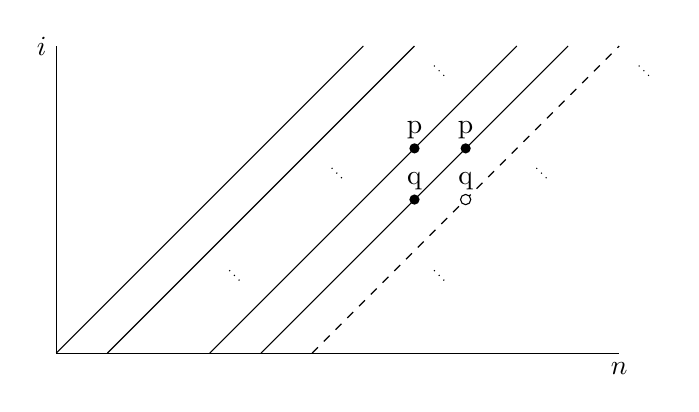
\begin{tikzpicture}[scale = .65]
	\draw (0,0)--(0,6);
	\draw (0,0)--(11,0);
	\draw (0,0)--(6,6);
	\draw (1,0)--(7,6);
	\draw (3,0)--(9,6);
	\draw (4,0)--(10,6);
	\draw[dashed] (5,0)--(11,6);

	\draw[dotted, shorten >=10pt,shorten <=10pt] (3,2)--(4,1);
	\draw[dotted, shorten >=10pt,shorten <=10pt] (5,4)--(6,3);
	\draw[dotted, shorten >=10pt,shorten <=10pt] (7,6)--(8,5);

	\fill (7,4) circle (0.1);
	\fill (8,4) circle (0.1);
	\fill (7,3) circle (0.1);
	\fill[white] (8,3) circle (0.1);
	\draw (8,3) circle (0.1);

	\node[above] at (7,4) {p};
	\node[above] at (8,4) {p};
	\node[above] at (7,3) {q};
	\node[above] at (8,3) {q};

	\draw[dotted, shorten >=10pt,shorten <=10pt] (7,2)--(8,1);
	\draw[dotted, shorten >=10pt,shorten <=10pt] (9,4)--(10,3);
	\draw[dotted, shorten >=10pt,shorten <=10pt] (11,6)--(12,5);

	\node[below] at (11,0) {$n$};
	\node[left] at (0,6) {$i$};
	\end{tikzpicture}
	\caption{Representation of the implication in \cref{l:induction step} serving as the induction step in the proof of \cref{t:main}.}
	\label{f:induction step}
\end{figure}

\begin{lemma}\label{l:induction step}
	Let $\big\{ \triangle_i [n] \big\}_{i,n\in\N}$ be a free non-degenerate and irreducible \mbox{cup-$i$} construction.
	Let $\big\{ \p(i,n) \big\}_{i,n \in \N}$ and $\big\{ \q(i,n) \big\}_{i,n \in \N}$ each be one of the following two families of propositions:
	\[
	\big\{ \triangle_i [n] = \Delta_ i [n] \big\}_{i,n \in \N}
	\quad \text{or} \quad
	\big\{ \triangle_i [n] = T \Delta_ i [n] \big\}_{i,n \in \N} \ .
	\]
	For all $i,n \in \N$ with $i \leq n-2$ the following implication holds:
	\[
	\boxed{\p(i+1,n) \wedge \p(i+1,n-1) \wedge \q(i,n-1)}\ \Longrightarrow\ \boxed{\q(i,n)}
	\]
\end{lemma}

\begin{proof}
	Let both $\big\{ \p(i,n) \big\}_{i,n\in\N}$ and $\big\{ \q(i,n) \big\}_{i,n\in\N}$ be the family $\big\{ \triangle_i [n] = \Delta_i [n] \big\}_{i,n \in \N}$.
	The other three combinations are treated analogously.

	From $\p(i+1,n)$ and $\p(i+1,n-1)$ we have
	\[
	\bd \triangle_{i+1} [n] + \triangle_{i+1} \bd \, [n] =
	\bd \Delta_{i+1} [n] + \Delta_{i+1} \bd \, [n]
	\]
	or, equivalently,
	\begin{align*}
	(1+T) \triangle_i [n] =
	(1+T) \Delta_i [n] \defeq
	(1+T) \sum_{\mathclap{U \in \P_{n-i}^n}} {U^0} \ot {U^1}
	\end{align*}
	\cref{l:consequence} implies the existence of a function $\xi \colon \rP_{n-i}^n \to \Ftwo$ such that
	\[
	\triangle_i [n] =
	\sum_{\mathclap{U \in \P_{n-i}^n}} U^\xi \ot U^\barxi.
	\]
	\cref{l:first nail} implies, using $\q(i,n-1)$, that
	\[
	\triangle_i [n] = \Delta_i [n]
	\quad \text{or} \quad
	\triangle_i [n] = T \Delta_i [n].
	\]
	Finally, \cref{l:second nail} implies $\triangle_i [n] = \Delta_i [n]$, i.e., $\q(i,n)$.
\end{proof}

\subsection{Complete proof}\label{ss:proof}

We now present the proof of our main result.

\begin{proof}[Proof of \cref{t:main}]
	Let $\big\{ \triangle_i [n] \big\}_{i,n\in\N}$ be a non-degenerate, irreducible, and free \mbox{cup-$i$} construction.
	We will use an induction argument over $k = n-i$ to show that for each $i \in \N$ either $\triangle_i [n] = \Delta_i [n]$ or
	$\triangle_i [n] = T \Delta_i [n]$ for all $n \in \N$.
	By \cref{l:special case one} $\triangle_i [n] = \Delta_i [n]$ and $\triangle_i [n] = T \Delta_i [n]$ for $r \leq 0$.
	By \cref{l:special case two} $\triangle_i [n] = \Delta_i [n]$ or $\triangle_i [n] = T \Delta_i [n]$ for $r = 1$.
	This serves as the base case of the induction and \cref{l:induction step} as the induction step (\cref{f:induction step}).
\end{proof}